% ----------------------------------------------------------------------
%
%                          TFG.tex
%
%----------------------------------------------------------------------

\documentclass[11pt,a4paper,twoside]{book}

\usepackage[spanish]{babel}

%paquete para crear links
\usepackage[breaklinks=true]{hyperref}

%paquete para usar urls
\usepackage{url}

%paquete para insertar imagenes
\usepackage{graphicx}

%paquete para insertar animaciones con imagenes
\usepackage{animate}

% Incluimos el fichero con comandos de constantes
%---------------------------------------------------------------------
%
%                          constantes.tex
%
%---------------------------------------------------------------------
%

%Título del documento
\def\titulo{Uso de VR y AR para el entrenamiento de actividades físicas }

\def\autor{Raúl Fernández Pérez}

\def\institucion{Departamento de Ingeniería del Software e Inteligencia Artificial\\[0.2em]
Facultad de Informática\\[0.2em]
Universidad Complutense de Madrid \\[1em]
Septiembre 2020 }

\def\tutor{Gonzalo Méndez Pozo, Pablo Gervás Gómez-Navarro}

\def\tfg{Trabajo de Fin de Grado}

%paquete para utiliar el simbolo del euro
\usepackage{eurosym} 

%paquete para tabla
\usepackage{multirow}

%paquete para la cabecera de las páginas
\usepackage{fancyhdr}
\usepackage{emptypage}

%paquete para utilizar una bibliografia 
\usepackage[maxbibnames=99, sorting=none, backend=bibtex]{biblatex}
\addbibresource{referencias.bib}

% Sacamos en el log de la compilación el copyright
\typeout{Copyright Raúl Fernández Pérez}

\graphicspath{{Imagenes/} }

\usepackage{float}


%%%%%%%%%%%%%%%%%%%%%%%%%%%%% Documento %%%%%%%%%%%%%%%%%%%%%%%%%%%%%%%%%%
\begin{document}

%estilo de la cabecera
\pagestyle{fancy}
\fancyhf{}
\renewcommand{\headrulewidth}{0pt}

%Nivel hasta que muestra los epigrafes
\setcounter{secnumdepth}{3} 

%Numeración romana
\frontmatter

%---------------------------------------------------------------------
%
%                            Portada.tex
%
%---------------------------------------------------------------------
%
% Fichero que contiene la portada y las 2 primeras hojas del TFG


\begin{titlepage}
    \begin{center}

        {\huge\textbf{ \titulo \\[1em]} \par } 

        \begin{figure}[h]
            
\includegraphics[scale = 0.3]{escudoUCM}
            \centering \\[3em]
        \end{figure} 

        \textbf\tfg \\[1em]

        \textbf\autor \\[1em]

        \textbf\institucion
        

    \end{center}
\end{titlepage}

%%%%%%%%%%%%%%%%%%%%%%%%%%%%%%  Apendice  %%%%%%%%%%%%%%%%%%

\cleardoublepage 

\begin{center}
    
    {\huge\titulo}
    
    \vspace{4cm}

    \textit\tfg \par
    \textbf{Ingeniería del Software e Inteligencia Artificial} \\[2em]

    \textit{Dirigido por los Doctores} \par
    \textbf\tutor

    \vspace{4cm}
    \textbf\institucion
\end{center}






%---------------------------------------------------------------------
%
%                      dedicatoria.tex
%
%---------------------------------------------------------------------



\chapter*{Dedicatoria}
\addcontentsline{toc}{chapter}{Dedicatoria}

\begin{center}
\textit{A mis familiares por darme todo y apoyarme para conseguir siempre lo que me proponga\\[1em]
A mi novia Ana, por su apoyo y siempre alentarme a ser mejor\\ [1em]
A todos mis amigos que me han acompañado y ayudado todo este tiempo\\[1em]
A todos ellos le dedico este trabajo porque sin ellos no habría sido posible}

\end{center}
%---------------------------------------------------------------------
%
%                      agradecimientos.tex
%
%---------------------------------------------------------------------


\chapter*{Agradecimientos}
\addcontentsline{toc}{chapter}{Agradecimientos}


\textit{Quisiera agradecer a Gonzalo Méndez Pozo y a Pablo Gervás Gómez-Navarro, los directores de este trabajo, por todo el apoyo que me han proporcionado para realizarlo.}

\textit{También me gustaría agradecer a los miembros de mi familia, mis padres y amigos que me han mostrado su apoyo y ánimos durante la creación de este trabajo.}

\textit{A mi amiga de la infancia Ana Galindo Lobato por su dedicación, gracias por ayudarme a llegar tan lejos, sin ti no lo hubiera conseguido.}

\textit{Esto va también por vosotros frescos(SOF), mis grandes hermanos.}

\textit{También quería agradecérselo a esa persona que me hace la vida más fácil cada día, a mi novia Ana.}



%---------------------------------------------------------------------
%
%                      resumen.tex
%
%---------------------------------------------------------------------


\chapter*{Resumen}
\addcontentsline{toc}{chapter}{Resumen}

Este proyecto tiene como meta el diseño, desarrollo y despliegue de un entrenador personal virtual mediante la captura de movimiento utilizando la tecnología de realidad virtual y realidad aumentada.
Con el objetivo de entender y abordar de una manera correcta este proyecto, se han revisador diferentes tecnologías existentes en el mercado para el desarrollo de un sistema capaz de captura los movimientos en tiempo real. Se han expuesto las ventajas que han llevado a utilizar dispositivos de \textit{VR}, mencionando diferentes estudios previos con resultados satisfactorios. Además, se han detallado las novedades que aportan las diferentes soluciones existentes en la danza, los entrenadores personales o las artes marciales, en el ámbito de los \textit{Reactive Virtual Trainers (RVT)}.
Este proyecto presenta un sistema para el entrenamiento personal de un arte marcial brasileño (capoeira), el cual se define como una mezcla entre los deportes de danza y lucha. El entorno desarrollado está pensado para que el alumno pueda practicar y perfeccionar diferentes movimientos sobre capoeira sin la necesidad de que un profesor revise sus movimientos.
Para la realización del entrenamiento, es necesario imitar una serie de movimientos grabados previamente por expertos en el arte marcial. Para que el alumno pueda avanzar en la realización de los movimientos, existen diferentes niveles de entrenamiento donde el alumno va aprendiendo de forma progresiva.
El sistema es capaz de adaptarse fácilmente para, por ejemplo, la medicina deportiva o la rehabilitación de alguna parte del cuerpo dañada.
Tras el estudio realizado, se pudo observar que el funcionamiento de las aplicaciones es inmersivo, intuitivo y rápido, ofreciendo un sistema amplio para 
determinar de una forma visual cuales son los movimientos ejecutados de forma errónea. Por todo ello, se puede afirmar que este tipo de sistemas son el presente y futuro para el aprendizaje en diferentes disciplinas.




Palabras clave:Mocap, captura de movimiento, Reactive Virtual Trainer, RVT, Unity, entrenador personal, Vr y AR.

%---------------------------------------------------------------------
%
%                      abstract.tex
%
%---------------------------------------------------------------------


\chapter*{Abstract}
\addcontentsline{toc}{chapter}{Abstract}


The target of this Project is developing

%indice
\tableofcontents

%indice de figuras
\listoffigures

%Numeración de las páginas
\mainmatter

%estilo de la cabecera para los capitulos
\lhead[\leftmark]{\thepage}
\rhead[\thepage]{\rightmark}
\addtolength{\headheight}{2pt}
\renewcommand{\headrulewidth}{0.5pt}


%---------------------------------------------------------------------
%
%                          Capítulo 1
%
%---------------------------------------------------------------------



\chapter{Introducción}
\label{cap1:sec:introduccion}

En la actualidad los sistemas de captura de movimiento 


\section{Objetivos del trabajo}

\section{Plan de Trabajo}

\section{Estructura de la memoria}



%---------------------------------------------------------------------
%
%                          introduction.tex
%
%---------------------------------------------------------------------


%\addtocounter{chapter}{-1} 
\chapter{Introduction}
\label{cap2:sec:introduction}

En la actualidad los sistemas de captura de movimiento 


\section{Objetivos del trabajo}

\section{Plan de Trabajo}

\section{Estructura de la memoria}

%---------------------------------------------------------------------
%
%                          capítulo 3
%
%---------------------------------------------------------------------



\chapter{Estado del arte}

\section{Captura de movimiento}
\label{cap3:sec:capitulo3}

Los sistemas de captura de movimiento o \texttt{Mocap}, son un conjunto de técnicas que se utilizan para registrar los movimientos, ya sea de objetos, animales o mayormente personas, trasladándolos a un modelo 3D.
En la actualidad, esta técnica se utiliza en la industria del cine y de los videojuegos ya que facilita mucho la labor de los animadores al realizar un modelado más realista. En el cine se utiliza como mecanismo para almacenar los movimientos realizados por los actores, y así poder animar los modelos 3D de los diferentes personajes que tenga el film. En cambio, en el sector de los videojuegos se utiliza para naturalizar los movimientos de los personajes. De ese modo se obtiene una mayor sensación de realismo.

\section{Historia de la captura de movimiento}

\subsection{Precursores}
Ya en la antigua Grecia, Aristóteles (384-322 AC) escribió el libro \textit{``De Motu Animalium''} (Movimiento de los animales). El no solo veía los cuerpos de los animales como sistemas mecánicos, sino que perseguía la idea de cómo diferenciar la realización de un movimiento y como poderlo hacer realmente, por lo que podrá ser considerado el primer biomecánico de la historia.

Aproximadamente dos mil años después, Leonardo da Vinci (1452-1519) trató de describir algunos mecanismos que utiliza el cuerpo humano para poder desplazarse, como un humano puede saltar, caminar, mantenerse de pie, etc.

Como pionero en la edad moderna, Eadweard Muybridge (1830-1904) fue el primer fotógrafo capaz de diseccionar el movimiento humano y animal, a través de múltiples cámaras tomando varias fotografías para captar instantes seguidos en el tiempo. Este experimento llamado ``el caballo en movimiento'', (véase Figura \ref{fig:EadweardMuybridgeHorse}),  utiliza esta técnica de fotografía. \cite{Mejias2014} \cite{Menendez2015}


\begin{figure}[h!]
    \centering
    \animategraphics[loop,autoplay,width=0.8\linewidth]{10}{/EadweardMuybridge/EadweardMuybridge-}{0}{14}
    \caption{El caballo en movimiento de Eadweard Muybridge}
    \label{fig:EadweardMuybridgeHorse}  
\end{figure}


\subsection{Nacimiento de la captura de movimiento}

Al principio de la industria cinematográfica, en la década de 1970, cuando empezaba a surgir la posibilidad de realizar animaciones de personajes por ordenador, se conseguía naturalizar los movimientos mediante técnicas clásicas de diseño, como la técnica de rotoscopia. 
Esta técnica consiste en reemplazar los frames de una grabación real por dibujos calcados en cada frame. Los estudios \textit{Walt Disney Pictures} utilizaron esta técnica en la película de 1937 ``Blancanieves y los siete enanitos'' (véase Figura \ref{fig:Blancanieves}),  para animar a los personajes del príncipe y Blancanieves. 

\begin{figure}[h!]
    \centering
    \animategraphics[loop,autoplay,width=0.8\linewidth]{10}{/Blancanieves/Blancanieves-}{0}{24}
    \caption{Rotoscopia en la película Blancanieves y los siete enanitos}
    \label{fig:Blancanieves}  
\end{figure}

En la década de 1980, en los laboratorios de biomecánica hubo un crecimiento en el análisis del movimiento humano mediante el uso de ordenadores. \texttt{Tom Calvert}, profesor de kinesióloga y ciencias de la computación en la universidad Simon Fraser (Canadá), fue uno de los primeros en usar potenciómetros para rastrear los movimientos del cuerpo humano, con el objetivo de ser utilizados por estudios coreográficos y asistencia clínica para ayudar a pacientes con problemas de locomoción.

Mientras tanto surgen los primeros sistemas de monitoreo visual, centros como el MIT (Massachusetts Institute of Technology) empezaron a realizar experimentos con dispositivos de seguimiento visual aplicados en el cuerpo humano. Mas tarde, empiezan a cobrar importancia los primeros sistemas de seguimiento visual como el \texttt{Op-Eye} y el \texttt{SelSpot}. Estos sistemas normalmente usaban pequeños marcadores adheridos al cuerpo (Leds parpadeantes) con una serie de cámaras alrededor del espacio donde se realizaba la actividad.

En 1988, Brad deGraf y Wahrman desarrollaron \textit{Mike the Talking Head} de Silicon Graphics, capaz de mostrar las capacidades de sus nuevos equipos 4D en tiempo real. Mike estaba dirigido por un controlador que permitía controlar diferentes parámetros de la cara del personaje: como los ojos, boca, expresión y posición de la cabeza. El hardware de Silicon Graphics proporcionaba una interpolación en tiempo real entre las expresiones faciales y la geometría de la cabeza del personaje y del usuario. En el congreso de SIGGRAPH, Mike fue mostrado al público, donde se demostró que la tecnología \textit{mocap} estaba preparada para su explotación. 

Tras estos avances, Pacific Data Images desarrolló un exoesqueleto de plástico, de modo que el actor se colocaría el traje con el objetivo de capturar los movimientos corporales: de la cabeza, pecho y brazos, a través de potenciómetros situados en la capa de plástico. De esta manera, los actores podrían controlar los personajes virtuales mimetizando sus movimientos. Pese a que el traje se utilizó en varios proyectos, no se consiguieron los resultados esperados, ya que el ruido de los circuitos y el diseño inapropiado del traje no lo permitían. 

En torno a 1992, la empresa SimGraphics desarrolló un sistema de rastreo facial llamado \textit{Face Waldo}. Consiguieron capturar la mayor parte de los movimientos usando sensores adheridos a la barbilla, labios, mejillas, cejas y en el armazón del casco que llevaba el actor para su posterior aplicación en un personaje virtual en tiempo real. Este sistema logró ser novedoso ya que el actor podía manejar las expresiones faciales de un personaje a través de sus movimientos, logrando unos gestos más naturales que los capturados anteriormente.

Lo que produjo un éxito mayúsculo con este proyecto fue la interpretación en tiempo real de Mario, el personaje principal de la saga de videojuegos \textit{Mario Bros}. Estaba controlado por un actor mediante \textit{Face Waldo}, Mario conseguía dialogar con los miembros de una conferencia, respondiendo a sus preguntas. A partir de ese momento, SimGraphics se centró en la animación en directo, desarrollando personajes para televisión y otros eventos en directo, mejorando la fiabilidad del sistema para el rastreo facial. 

De forma gradual, la técnica \textit{mocap} se fue expandiendo entre las empresas desarrolladoras de sistemas de captura de movimientos, con el objetivo de crear productos y métodos que albergasen nuevos sectores empresariales. 

A lo largo de la última década, hemos visto como han ido apareciendo largometrajes que iban mostrando la evolución de la captura de movimiento con una gran proyección de futuro. Ha pasado de ser una técnica que se utilizaba de forma esporádica para algunos personajes, ha ser indispensable en cualquier producción. Como por ejemplo en los\textit{films}: Gollum en la trilogía de El Señor de los Anillos y de El Hobbit, Avatar, El planeta de los simios, Los vengadores (véase Figura \ref{fig:Thanos}) entre otros. De igual modo, esta técnica es muy utilizada actualmente en los videojuegos como, por ejemplo: The Last Of Us (véase Figura \ref{fig:TheLastOfUs}), Fifa 20, Red Dead Redemption, Uncharted 4.

\begin{figure}[h!]
    \centering
    \animategraphics[loop,autoplay,width=0.8\linewidth]{10}{/Thanos/Thanos_}{0}{19}
    \caption{Mocap en la película Los vengadores}
    \label{fig:Thanos}  
\end{figure}

\begin{figure}[h!]
    \centering
    \animategraphics[loop,autoplay,width=0.8\linewidth]{10}{/TheLastOfUs/TheLastOfUs-}{0}{103}
    \caption{Mocap en el videojuego The Last Of Us}
    \label{fig:TheLastOfUs}  
\end{figure}


\section{Métodos de captura de movimiento}

En la actualidad existen numerosos sistemas de captura de movimiento. Dependiendo de las necesidades de la producción, ya estén relacionados con el presupuesto disponible, así como las posiciones, velocidades, impulsos del actor o el nivel de realismo al que se quiera llegar. Atendiendo a las tecnologías más utilizadas en la actualidad para la captura de movimiento, se desglosan dos grandes grupos: los sistemas ópticos y no ópticos (incluyendo magnéticos, mecánicos, e inerciales).

Los sistemas ópticos funcionan mediante el seguimiento de marcadores físicos, como luces LED, reflectores, adhesivos con apariencia de pelota de ping-pong o incluso simplemente pintura facial.

Los sistemas no ópticos no utilizan ningún tipo de marcador físico. En su lugar, utilizan software de movimiento de fósforos para seguir el movimiento de un actor, pero este software funciona identificando características clave de un humano, como la boca o una prenda de vestir. Los directores de fotografía crean un boceto rápido en gráficos por ordenador de cualquier personaje que quieran dar vida, y mapean el esqueleto del personaje en el metraje de acción en vivo, teniendo en cuenta la posición, la escala, la orientación y el movimiento.

Esto es mucho más asequible ya que se basa principalmente en software y no requiere de tanto hardware. En un plató para grabar una película o un videojuego, primero se crea el personaje animado digitalmente y, mientras se graba, pueden mapear este personaje sobre el actor mediante captura de movimiento, para que puedan ver instantáneamente cómo el movimiento se traduce en el personaje, junto con la iluminación y los ángulos preferidos. Esto se conoce como cinematografía virtual.

Atendiendo a su tecnología, se pueden encontrar los diferentes métodos que se desarrollan a continuación.

\subsection{Captura de movimiento no óptico}

\subsubsection{Captura de movimiento magnético}

Los sistemas de captura de movimiento magnéticos están formados por sensores creados por tres espirales ortogonales que miden el flujo magnético, determinando tanto la posición como la orientación del sensor. Un transmisor genera un campo electromagnético de baja frecuencia que los receptores detectan y transmiten a la unidad electrónica de control, donde se filtra y amplifica. A continuación, los datos se envían a un ordenador central, donde se deduce la orientación y posición de todos los sensores del escenario. 

Un sistema magnético estándar consta de 18 sensores, una unidad de control electrónica y un software para el procesamiento. En cambio, un sistema de última generación puede tener hasta 90 sensores capaces de capturar hasta 144 muestras por segundo, teniendo un coste medio (en torno a 6.000 \euro).

Estos sistemas tienen el inconveniente de producir interferencias con materiales metálicos debido a su conductividad, ya que se crean campos magnéticos que interfieren con el campo magnético del emisor. De ese modo, se trata de un sistema difícil de transportar a diferentes escenarios. El proceso de captura no es en tiempo real, aunque se aproxima bastante, pese a que tiene un número de capturas por segundo demasiado bajo. Como punto a favor, es más fácil procesar los datos que en otros sistemas \textit{mocap}, ya que los datos obtenidos están en relación con la posición del actor.


\subsubsection{Captura de movimiento mecánico}

En el proceso de captura de movimiento mecánica el actor viste unos trajes especiales adaptables al cuerpo humano. En su mayoría, estos trajes están compuestos por estructuras rígidas con barras metálicas o plásticas, unidas mediante potenciómetros colocados en las principales articulaciones. Los potenciómetros se componen de un elemento deslizante acoplado a una resistencia, la cual produce una variación de tensión que puede medirse para conocer el grado de apertura de la articulación donde se encuentre acoplado. Los sensores que recogen la información pueden transmitirla mediante cables, pero normalmente lo hacen con radiofrecuencia.

Estos sistemas tienen el problema de que son incapaces de medir translaciones globales. Pueden medir posiciones relativas de los miembros, pero no como se desplaza el actor por el escenario. Además, el único valor que utilizan para medir es el grado de apertura, no teniendo en cuenta rotaciones complejas que poseen las articulaciones humanas, como es el caso de los hombros, cadera, tobillos, etc. También tienen el inconveniente de ser pesados, restringir el movimiento del actor y su corto tiempo de vida. En cambio, tienen la ventaja de tener un coste relativamente bajo (en torno a 30.000 \euro), capaz de registrar los movimientos del actor en tiempo real con un alcance mayúsculo. 

\subsubsection{Captura de movimiento inercial}

Con el objetivo de capturar el movimiento, los sistemas inerciales se basan en el sistema vestibular humano, el cual regula el sentido de movimiento y del equilibrio, es lo que nos permite situar nuestro cuerpo en el espacio, los desplazamientos y nuestro entorno. El sistema vestibular, ubicado en el oído interno, es un sensor inercial 3D biológico, ya que puede detectar el movimiento angular y la aceleración lineal de la cabeza, permitiendo por su actividad sobre el ojo conservar una imagen estable en la retina. 

Un giroscopio de velocidad mide la velocidad angular y, si se integra con el tiempo, proporciona el cambio de ángulo con respecto a un ángulo inicialmente conocido. Un acelerómetro mide las aceleraciones, incluida la aceleración gravitacional \textit{g}. Si se conoce el ángulo del sensor con respecto a la vertical, se puede eliminar el componente de gravedad y, mediante integración numérica, se pueden determinar la velocidad y la posición

De este modo, con la información obtenida de los sensores, esta se transmite a un ordenador, donde se puede observar el movimiento capturado sobre una figura ya animada. Este tipo de sistemas no utiliza mecanismos externos como cámaras; y como en el caso de los sistemas ópticos, cuantos más sensores se utilicen, más real será el movimiento capturado, teniendo unos grandes rangos de captura. 


\subsection{Captura de movimiento óptico}

La detección de movimiento óptico abarca una amplia y variada colección de tecnologías. Los sistemas basados en imágenes determinan la posición mediante el uso de varias cámaras para rastrear puntos predeterminados (marcadores) en los segmentos del cuerpo del actor, alineados con puntos de referencia óseos específicos. La posición se estima mediante el uso de múltiples imágenes 2D del volumen de trabajo. Las técnicas estereométricas correlacionan puntos de seguimiento comunes en los objetos rastreados en cada imagen y utilizan esta información junto con el conocimiento sobre la relación entre cada una de las imágenes y los parámetros de la cámara para calcular la posición.

Estos sistemas permiten la grabación en tiempo real, ya que utilizan un ordenador que recibe la entrada de una o más cámaras digitales CCD (\textit{Charge-coupled device}) sincronizadas produciendo proyecciones simultáneas. Habitualmente se utilizan en torno a 4 o 32 cámaras, siempre y cuando no se añadan de forma innecesarias, ya que complicarían el procesamiento de la información.

Las cámaras utilizadas en este tipo de sistemas tienen una velocidad de captura de entre 30 y 1.000 fotogramas por segundo. Estos sistemas se deben calibrar mediante el rastreo de un objeto visible, de modo que se calcule la posición de cada cámara respecto de ese punto, en el caso de que una cámara se mueva, sería necesario recalibrar el sistema. La interferencia de otras fuentes de luz o reflejos también puede ser un problema que puede resultar en los llamados marcadores fantasma.

Existen varias clases de sensores para este tipo de captura de movimiento:

\subsubsection{Marcadores activos}

Este sistema está compuesto por leds que emiten su propia luz para crear un plano de luz que atraviesa la imagen determinando la posición del actor, de esta manera se consigue aumentar la distancia a la que se puede desplazar el artista. La posición de los marcadores se determina iluminando uno o varios indicadores, de manera sincrónica a las cámaras en cada instante de tiempo, a una frecuencia de muestreo muy alta. De modo que los indicadores deben estar sincronizados con todas las cámaras para realizar una sola captura en cada iluminación. 

Son más apropiados para aplicaciones de mapeo que para el seguimiento dinámico de movimiento del cuerpo humano. Este tipo de sistemas ópticos sufren problemas de oclusión (línea de visión) cuando se bloquea una trayectoria de luz requerida por el sistema.

\subsubsection{Marcadores pasivos}

Los sistemas ópticos con marcadores pasivos utilizan LED de infrarrojos (IR) montados alrededor de la lente de la cámara, junto con filtros de paso de infrarrojos colocados sobre la lente de la cámara y miden la luz reflejada por los marcadores. De esta forma, la luz que reflejan se origina cerca de las cámaras, siendo recogida por estas. 

Los sistemas ópticos basados en LED de pulso miden la luz infrarroja emitida por los LED colocados en las partes del cuerpo. Además, es posible el seguimiento de objetos naturales mediante una cámara sin la ayuda de marcadores, pero en general es menos preciso. Se basa en gran medida en técnicas de visión por ordenador para el reconocimiento de patrones y, a menudo, requiere grandes recursos computacionales. Este tipo de sistemas pueden capturar un gran número de marcadores a una frecuencia de muestreo de hasta 2000 fotogramas por segundo. Se suelen utilizar principalmente para el registro de movimiento facial. 

\section{Métodos de captura de movimiento emergentes}

En la actualidad, el sector cinematográfico y la industria de los videojuegos ha generado la necesidad de crear personajes con gestos y movimientos más realistas, de este modo, se ha conseguido que la captura de movimiento se convierta en una herramienta esencial, ya que permite una mayor inmersión. 

Gracias a estos sectores, han surgido nuevas técnicas de \textit{Motion Capture}, en la que cámaras y software de inteligencia artificial pueden realizar un enfoque de captura de movimiento sin la necesidad de marcadores. El software permite que, mediante algoritmos, se analice al usuario que realiza las acciones, identificando formas humanas, movimientos, expresiones y gestos.


\subsection{Visión artificial}

La visión artificial \cite{Visionartificial} es una disciplina científica que incluye métodos para adquirir, procesar, analizar y comprender las imágenes del mundo real con el fin de producir información numérica o simbólica para que puedan ser tratados por un ordenador. Tal y como los humanos usamos nuestros ojos y cerebros para comprender el mundo que nos rodea, la visión artificial trata de producir el mismo efecto para que los ordenadores puedan percibir y comprender una imagen o secuencia de imágenes y actuar según convenga en una determinada situación. Actualmente se está utilizando cada vez más para el análisis y tratamiento de imágenes mediante algoritmos de inteligencia artificial. 

Atendiendo a su demanda, se pueden encontrar diferentes tecnologías que se desarrollan a continuación.

\subsubsection{Microsoft Azure Kinect DK}

Previamente al actual dispositivo \textit{Azure Kinect DK} (véase Figura \ref{fig:AzureKinectDK}), Microsoft en 2010 desarrolló \textit{Kinect} para \textit{Xbox-One}, un dispositivo pensado para su uso en los videojuegos. Este periférico prescinde de mandos gracias a que dispone de una cámara RGB, un sensor de profundidad, un proyector de luz infrarroja, un micrófono bidireccional y un procesador que utiliza algoritmos para procesar las imágenes tridimensionales.

\begin{figure}[h!]
    \centering
    \animategraphics[loop,autoplay,width=0.7\linewidth]{10}{/AzureKinectDK/AzureKinectDK_}{0}{46}
    \caption{Azure Kinect DK}
    \label{fig:AzureKinectDK}   
\end{figure}



En marzo de 2020, Microsoft actualizó su dispositivo a la versión \textit{Azure Kinect DK }\cite{AzureKinect}, se trata de un kit para desarrolladores con sensores de inteligencia artificial avanzados que proporcionan modelos sofisticados de visión y voz por ordenador. Este nuevo periférico contiene un sensor de profundidad, una matriz de micrófonos espaciales con una cámara de video y un sensor de orientación como un dispositivo pequeño todo en uno con múltiples modos, opciones y kits de desarrollo de software (SDK) con un gran potencial que se pueden conectar a Azure Cognitive Services, Azure Machine Learning y Azure IoT Edge.

Para localizar los movimientos de los objetos 3D, el periférico, transmite una luz infrarroja a través del escenario, lo que permite conocer el tiempo que tarda la luz en ser reflejada por los objetos. El sistema actúa como un sonar, determinando el tiempo que tarda en reflejarse la luz, estableciendo la distancia a la que se encuentran los objetos en tiempo real.


\subsubsection{OpenCV}

\textit{Open Source Computer Vision}\cite{OpenCV} comenzó como un proyecto de investigación en Intel. Actualmente es la biblioteca más popular de visión artificial, contando con implementaciones de más de 2500 algoritmos optimizados, que incluyen un conjunto completo de algoritmos de aprendizaje automático y visión por ordenador clásicos y de última generación. Estos algoritmos se pueden usar para detectar y reconocer rostros (véase Figura \ref{fig:OpenCV}), identificar objetos, clasificar acciones humanas en videos, rastrear movimientos de cámara, rastrear objetos en movimiento, extraer modelos 3D de objetos, producir nubes de puntos 3D a partir de cámaras estéreo, etc. Además, está disponible de forma gratuita para fines comerciales y de investigación.

\begin{figure}[h!]
    \centering
    \animategraphics[loop,autoplay,width=0.8\linewidth]{10}{/OpenCV/OpenCV_}{000}{021}
    \caption{Detección Facial con OpenCV }
    \label{fig:OpenCV}  
\end{figure}

\subsubsection{Deepfake}

Otro de los sistemas emergentes de visión artificial que utilizan el aprendizaje automático y la inteligencia artificial para manipular o generar contenido visual es el \textit{deepfake}. Se trata de una técnica que permite editar videos falsos de personas que aparentemente son reales (véase Figura \ref{fig:Obama}), utilizando para ello algoritmos de aprendizaje no supervisado, y videos o imágenes ya existentes. 

\begin{figure}[h!]
    \centering
    \animategraphics[loop,autoplay,width=0.8\linewidth]{10}{/Obama/Obama-}{0}{35}
    \caption{\textit{Deepfake} de Barack Obama}
    \label{fig:Obama}  
\end{figure}

Para crear un \textit{deepfake} \cite{Deepfake}, es necesario recopilar cientos de imágenes de las dos personas que queremos sustituir. Inicialmente se crea una codificación de todas las imágenes utilizando una red neuronal con \textit{deep learning}, posteriormente se utiliza un decodificador para reconstruir las imágenes, este proceso tiene un alto coste de procesamiento de GPU, necesitándose aproximadamente 3 días para generar resultados decentes (después de repetir el procesamiento de imágenes más de 10 millones de veces). Con todo ello se extraen las características más importantes para recrear la imagen original sustituyendo al usuario B con las características del usuario A en el video original.

Uno de los ejemplos más destacados del cine utilizando esta técnica es en la tercera saga de \textit{Star Wars}, donde en la película \textit{Rogue One una historia de Star Wars} la \textit{Princesa Leia} aparece con la cara de \textit{Carrie Fisher} cuando era joven, cuando en realidad fue interpretada por la actriz noruega \textit{Ingvild Deila} (véase Figura \ref{fig:Leia}). Años más tarde, la actriz falleció poco después de haberse completado el rodaje de la película \textit{Los últimos Jedi} y, contando con ella para aparecer en el \textit{Episodio IX - El ascenso de Skywalker}, fue necesario aplicar nuevamente las mismas técnicas para dar vida de nuevo a \textit{Carrie Fisher} como la \textit{Princesa Leia}.

\begin{figure}[h!]
    \centering
    \animategraphics[loop,autoplay,width=0.8\linewidth]{10}{/Leia/Leia_}{000}{031}
    \caption{\textit{Deepfake} de la Princesa Leia en Star Wars}
    \label{fig:Leia}  
\end{figure}

\subsection{Realidad virtual}

La realidad virtual es la tecnología que ofrece al usuario la sensación de estar en otro lugar, es decir, la tecnología engaña a tus sentidos, oculta el mundo real a tus ojos y te sumerge en uno nuevo de manera totalmente inmersiva. Se trata de una experiencia sensorial completa, simulando los espacios diversos en los que podemos explorar e interactuar el entorno tal y como si estuviéramos ahí realmente.

Para adentrarse en un entorno virtual, es necesario colocarse unas gafas especiales para poder visualizar la simulación, estas normalmente están conectadas a un ordenador, aunque ya existen modelos \textit{all in one}, aunque tienen la desventaja de no ser tan potentes gráficamente. 

Para determinar la posición exacta donde el usuario se encuentra situado tanto en el mundo real, como en el mundo virtual, estos sistemas vienen acompañados de unas estaciones base. Estos sensores son colocados en la habitación de juego permitiendo al sistema determinar la ubicación exacta tanto de las gafas de \textit{VR}, como de los controles y \textit{trackers}. 

Estos dispositivos de \textit{VR} disponen de sensores ópticos pasivos que reconocen el movimiento de tu cabeza, de manera que cuando la gires hacia un lado hagas el mismo movimiento dentro del mundo virtual en el que estés. 

Algunos modelos \textit{all in one} de \textit{VR} no necesitan estaciones base para determinar la posición en la que se encuentran los dispositivos de \textit{VR} en el entorno. Disponen de una serie de cámaras (véase Figura \ref{fig:Quest}) incorporadas en las mismas gafas de \textit{VR}, creando un sistema guardián que determina la zona de juego a utilizar en el mundo virtual.

\begin{figure}[h!]
    \centering
    \animategraphics[loop,autoplay,width=0.8\linewidth]{10}{/Quest/Quest_}{000}{021}
    \caption{Oculus Quest, modelo \textit{all in one} de \textit{VR}}
    \label{fig:Quest}  
\end{figure}

La producción de contenido de animación ha implicado tradicionalmente configuraciones de captura de movimiento muy caras que utilizan docenas de cámaras. Esta producción de animación de alta calidad estaba limitada a grandes estudios con grandes presupuestos. Pero en los últimos años, los avances en la tecnología de rastreo han traído una producción de animación de excelente calidad a proyectos de menor presupuesto, estudios de cine y juegos independientes. \cite{Vive}

Sin la necesidad de tener grandes equipos, surgen increíbles resultados con una excelente captura de movimiento (véase Figura \ref{fig:ViveMocap}).

\begin{figure}[h!]
    \centering
    \animategraphics[loop,autoplay,width=0.8\linewidth]{10}{/ViveMocap/ViveMocap_}{000}{066}
    \caption{Ejemplo de \textit{Mocap} con \textit{trackers} Vive}
    \label{fig:ViveMocap}  
\end{figure}

% \begin{figure}[h!]
%     \centering
%     \animategraphics[loop,autoplay,width=0.8\linewidth]{10}{/OculusRift/OculusRift-}{0}{52}
%     \caption{\textit{Hand tracking} en las Oculus Rift}
%     \label{fig:OculusRift}  
% \end{figure}

Como base para el estudio de la captura de movimientos y las tecnologías disponibles en este ámbito, se han realizado diferentes consultas a los siguientes proyectos: \cite{ Menendez2015} \cite{ Mejias2014} \cite{VIC}.

\section{Trabajo relacionado}

Para la realización de este proyecto se han revisado trabajos anteriores en el área de los \textit{Reactive Virtual Trainers}, además de cuáles son las tecnologías más emergentes en el mercado. En este apartado se describirán los análisis de esos proyectos, y de este modo, poder aclarar y enfocar el desarrollo de este proyecto.


% \subsection{Captura de movimiento en la danza}
% Uno de los campos en donde la captura de movimiento aparece es en la danza, y un claro ejemplo es \citep{Kyan:2015:ABD:2753829.2735951}. En este artículo se describe una forma de evaluar y visualizar en tiempo real, los movimientos de la danza de ballet. Para desempeñar esa tarea utilizan como recurso la tecnología de captura de movimiento \textit{Kinect}, y gracias a ella, registran los movimientos de bailarines profesionales, de modo que , sean una base para las comparaciones de movimientos. Estos, a su vez, son representados como un \textit{espacio de posturas} en forma de trayectorias de gestos. La evaluación de la coreografía empezaría cuando detecte al bailarín aficionado y con el fin de proporcionar una puntuación para cada coreografía, se compara la posición alineada y velocidad del bailarín aficionado con las correspondientes del bailarín profesional.


%---------------------------------------------------------------------
%
%                          capítulo 4
%
%---------------------------------------------------------------------

\chapter{Tecnologías empleadas}
\label{cap4:sec:capitulo4}

En este capítulo se presentan las tecnologías y dispositivos empleadas para el desarrollo del proyecto. Detallando de forma técnica el \textit{software} y \textit{hardware} utilizado.

\section{Software empleado}

Para el desarrollo de este proyecto, el principal software utilizado ha sido \texttt{Unity 2019.4.9f1}\cite{Unity_Manual}. Este \textit{Game Engine} hace referencia a una plataforma de desarrollo de software capaz de realizar rutinas de programación que permiten el diseño, la creación y el funcionamiento de un entorno interactivo;

Con el fin de elaborar, compilar y depurar el proyecto de \texttt{Unity} se ha utilizado \texttt{Visual Studio 2019}\cite{ VisualStudio} con el lenguaje de programación C\#, ya que mantienen una sola base de código para todas las plataformas. Respecto a la creación de los personajes, se observó que \texttt{Fuse Character Creator de Mixamo}\cite{FuseCharCreaMixamo} ofrecía una  creación de modelos humanos realistas con una alta calidad de las texturas. En cuanto a la configuración previa de las animaciones, se hizo uso de \texttt{Mixamo 3D Animation Online Services}\cite{Mixamo3DAnimation}, ya que es una compañía tecnológica encargada del desarrollo y venta de servicios para la animación de personajes 3D. Como plataforma para el desarrollo colaborativo del proyecto se usó GitHub, utilizando el sistema de control de versiones Git.

\subsection{Unity}
\label{cap4:sec:unity}

El objetivo de este proyecto trata de como poder realizar una captura de movimiento de calidad sobre el arte marcial afrobrasileño (capoeira) y como representarla gráficamente con las tecnologías más demandadas del mercado.

Un \textit{Game Engine} se especifica como la rutina de programación que permiten el diseño, la creación y la representación de un videojuego. La funcionalidad de un motor de videojuegos consiste en, proveer al desarrollador un motor de renderizado para la creación de gráficos 2D y 3D, un motor físico, sonidos, scripting, animaciones, un escenario gráfico, etc.

Para llevar todo esto a cabo es necesario elegir qué tipo de plataforma de \textit{Game Engine} utilizar en este proyecto. Existe dos grandes plataformas comerciales, por lo que la decisión de elegir entre \texttt{Unity}\footnote{\url{https://unity.com/}} o \texttt{Unreal Engine}\footnote{\url{https://www.unrealengine.com/}} fue basada en la comunidad que hay detrás de cada uno de ellos, y sobre todo, en lo que se quiere abarcar con este proyecto.

Además de este detalle, es importante conocer el lenguaje de programación con el que trabaja cada uno de ellos. \texttt{Unity} está basado en \texttt{C\#}, mientras que \texttt{Unreal Engine} trabaja con C++.

La versatilidad de \texttt{Unity}, ideal para proyectos pequeños, estudiantiles o enfocados al desarrollo de aplicaciones y juegos para móviles, ha conseguido que un 58\% de la población de desarrolladores indies lo elijan como motor de videojuegos. Las facilidades que aporta a la hora de trabajar de una forma visual y escalable lo convierten en un paso muy a tener en cuenta a la hora de realizar desarrollos enfocados a la creación de entornos 3D.

En este caso \texttt{Unity}, se adecua correctamente, ya que se pretende realizar un entorno 3D donde los usuarios perciban y aprendan movimientos del arte marcial afrobrasileño.

En un primer momento, \texttt{Unity} salió al mercado ofreciendo un \textit{software} de calidad y barato, añadiendo el objetivo de que pequeñas y grandes empresas pudieran utilizarlo por igual, dando además, la posibilidad de que su contenido sea compatible con prácticamente cualquier medio o dispositivo\cite{Unity-relations}. Gracias a ello, \texttt{Unity} creció exponencialmente en el mercado, generando así, una gran comunidad que puede servir de pilar de ayuda para los nuevos desarrolladores.

Como en otras plataformas de desarrollo de software, existen distintas licencias de prueba gratuitas y para estudiantes a las que puedes acceder sin complicaciones. Sólo aquél que realmente decida llevar su creación al mercado y supere cierta cantidad de ingresos se verá obligado a pagar la cuota mensual. En la versión personal (licencia gratuita), es necesario promocionar el logotipo de \texttt{Unity} cuando se inicia la aplicación una vez compilada.

Otro aspecto importante de \texttt{Unity} es el \texttt{Asset Store}. Se trata de una biblioteca, que contiene una multitud de paquetes o \textit{Assets} comerciales y gratuitos, creados de forma continua por la comunidad, por \texttt{Unity Technologies} o empresas de terceros. Estos paquetes pueden contener modelados 3D, texturas, animaciones y demás contenido que sirva de ayuda para desarrollar un proyecto donde ya sea por tiempo o habilidades técnicas, no sea posible desarrollar cada una de la herramientas que ofrece dicha tienda.

La plataforma para el desarrollo de este proyecto, \texttt{Unity},  está compuesta por varios paneles, cada uno de ellos representa información o acciones indispensables para el desarrollo del escenario 3D. La estructuración básica de un juego en \texttt{Unity} se realiza mediante escenas.  De modo que, para poder tener una previsualización de los elementos que aparecen en una escena, se utiliza el panel denominado \textit{Scene}, este panel representa una dimensión 3D, donde se podrán rotar y desplazar en los ejes de forma tridimensional, para conseguir de esta manera, modificar todos los elementos de la escena en cualquier Angulo.

El panel que muestra la vista generada por la cámara, es decir, la imagen que se verá cuando se reproduzca el juego se denomina \textit{Game}.

Los elementos incorporados a la escena, se archivan en otro panel, con el nombre \textit{Hierarchy}. Estos pueden ser modelos 3D, cámaras, prefabs(tipo de asset que te permite almacenar un objeto con componentes y propiedades preconfiguradas),sonidos, luces, e incluso objetos de tipo UI(\textit{buttons, sliders, toggles}) para la implementación de interfaces 2D. Los elementos se muestran de una forma jerárquica, al seleccionar uno, se expondrán sus características y componentes. En el panel, denominado \textit{Inspector}, al seleccionar un componente en el \textit{Hierarchy}, se muestra sus propiedades como el \textit{transform}, el cual muestra la información de su posición y rotación, pudiendo ser modificada.

Existe otro panel denominado \textit{Project}, donde se agrupan en forma de directorio, todos los \textit{scripts}, paquetes, modelos 3D, imágenes y archivos, relacionados con el proyecto.

Para comprobar el funcionamiento desarrollado en \textit{Unity} se necesita activar el \textit{Play mode}. Esta funcionalidad permite poner en funcionamiento el juego, pararlo y detener su ejecución, siendo esto, fundamental para comprobar y depurar un juego\cite{Unity_Manual}.

La transición de un script de Unity ejecuta una serie de funciones de eventos en un orden predeterminado. Este diagrama (véase Figura \ref{fig:UnityEvents}) describe algunas funciones de eventos y explica cómo encajan en la secuencia de ejecución dentro de la lógica del proyecto.


\begin{figure}[h]
    \centering 
    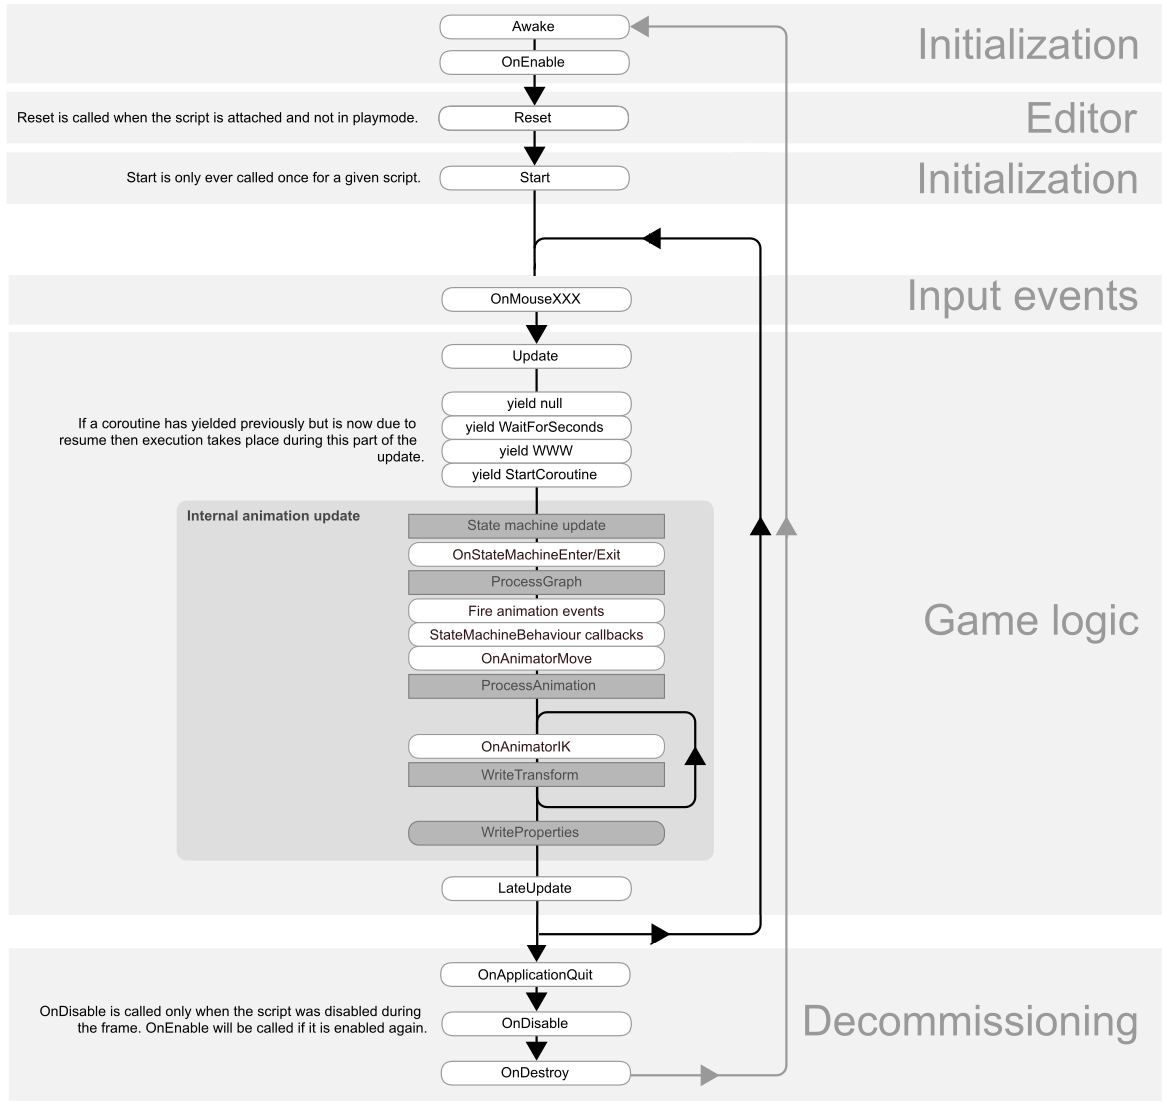
\includegraphics[scale = 0.4]{UnityEvents}
    \caption{Orden de ejecución para los eventos en Unity}
    \label{fig:UnityEvents} 
\end{figure} 

Las siguientes funciones, son algunas de las más importantes a la hora de desarrollar un escenario dentro de \textit{Unity}. Estas se llaman cuando una escena se ejecuta (una vez por cada objeto en la escena): 

\begin{itemize}
	\item \texttt{Awake}: esta función siempre se llama antes de cualquier función de inicio y también justo después de realizar una instancia de un \textit{prefab}.
 	\item \texttt{Start}: se llama al inicio antes de la actualización del primer marco solo si la instancia de secuencia de comandos está habilitada.
    \item \texttt{Update}: la actualización se llama una vez por fotograma. Es la principal función del motor para las actualizaciones de los \textit{frames}.
\end{itemize} 

Para construir todo el proyector de \textit{Unity} se utilizó el potente entorno de desarrollo \texttt{Visual Studio 2019}. 

\texttt{Visual Studio Tools} para \texttt{Unity} es una extensión gratuita de \texttt{Visual Studio} que convierte al editor en una poderosa herramienta para desarrollar juegos y aplicaciones multiplataforma con \texttt{Unity}.

Si bien el editor de \texttt{Unity} es excelente para crear el escenario 3D, pero no puedes escribir el código en él. Con \texttt{Visual Studio Tools} para \texttt{Unity}, se pueden usar las funciones familiares de edición, depuración y productividad de código para crear scripts en el proyecto de \texttt{Unity} usando C\#, pudiendo depurarlos usando las poderosas capacidades de depuración de \texttt{Visual Studio}.

Pero \texttt{Visual Studio Tools} para \texttt{Unity} es más que eso. También tiene una integración profunda con el editor de Unity para que dedique menos tiempo a realizar tareas simples, proporciona mejoras de productividad específicas de \texttt{Unity} y pone la documentación de al alcance de su mano.

\subsection{Adobe Fuse Character Creator}

Se trata de una aplicación desarrollada por Mixamo, la cual permite crear personajes 3D únicos mediante una intuitiva interfaz, separando el avatar en diferentes partes, como son la cabeza, el torso, las piernas y los brazos (véase Figura \ref{fig:AdobeFuse}). Posteriormente a la selección de las diferentes partes del cuerpo ya predefinidas por el sistema, se puede editar cada una de las partes del personaje, ya sean los rasgos de la cara, el tamaño de los brazos, la longitud de las piernas, etc. Al seleccionar la parte del cuerpo que se quiere modificar, simplemente sería necesario pinchar y realizar un \textit{scrool} o deslizamiento hacia la izquierda o derecha para aumentar su tamaño. Por otro lado, para seleccionar el punto exacto donde se ubicarán las diferentes partes del cuerpo como por ejemplo el ombligo, los ojos, las rodillas, etc, se realizará un \textit{scrool} o desplazamiento hacia arriba o abajo.

\begin{figure}[h!]
	\centering
	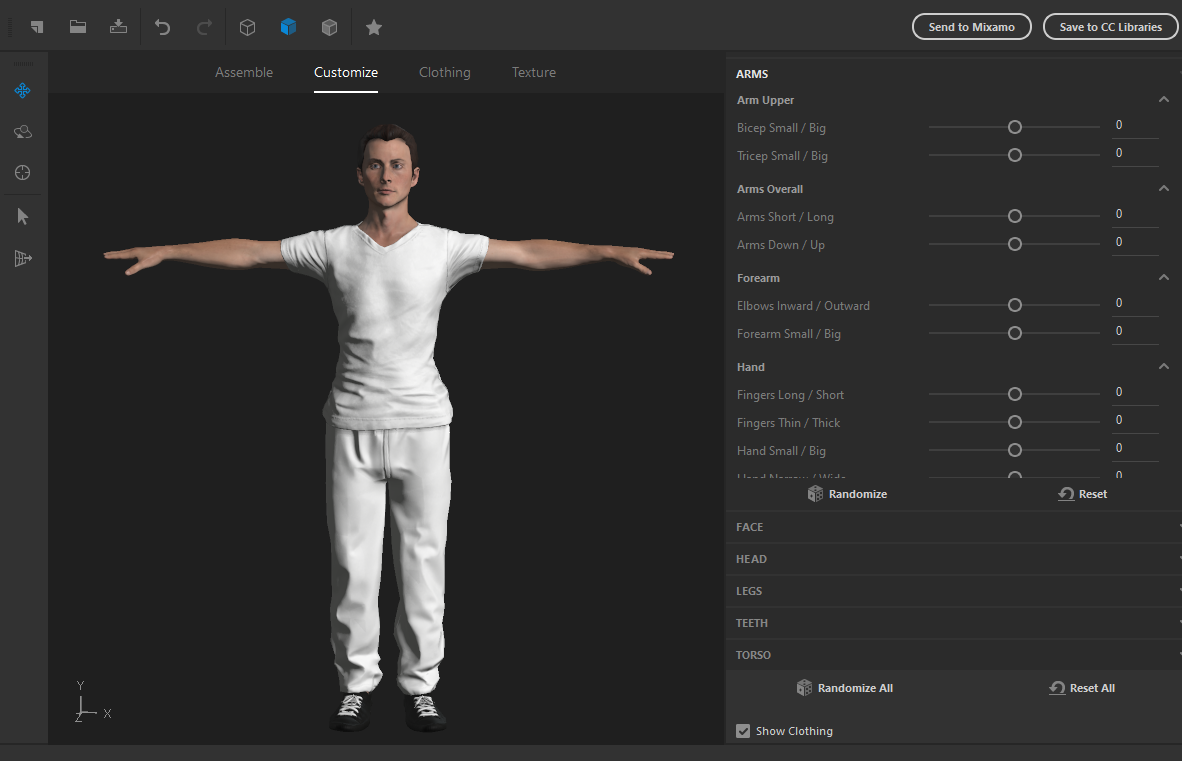
\includegraphics[scale = 0.4]{AdobeFuse}
	\caption{Configuración de un avatar con Adobe Fuse Character Creator}
	\label{fig:AdobeFuse}
\end{figure}

Al terminar de modelar el personaje, se pasará a la sección de vestuario. Donde existen prendas predefinidas, como camisas, pantalones, zapatos, etc. Al terminar de vestir al avatar, esta aplicación posee la peculiaridad de poder subir al servidor de Mixamo el modelado realizado \footnote{\url{https://www.adobe.com/es/products/fuse.html}}. Pudiendo completar la configuración de los huesos (\textit{rigger}), con la posibilidad de crear varios esqueletos para un mismo personaje y además incluir las animaciones deseadas.



\subsection{Mixamo}
\label{cap4:sec:mixamo}

Mixamo\footnote{\url{https://www.mixamo.com}} es una compañía tecnológica (adquirida en 2015 por Adobe System) encargada del desarrollo y venta de servicios para la animación de personajes 3D. Proporcionando un servicio \textit{online}, que permite buscar entre una amplia gama de movimientos, que van desde el combate, pasando por deportes, hasta poder tocar un instrumento (véase Figura \ref{fig:Mixamo}).

\begin{figure}[h]
    \centering 
    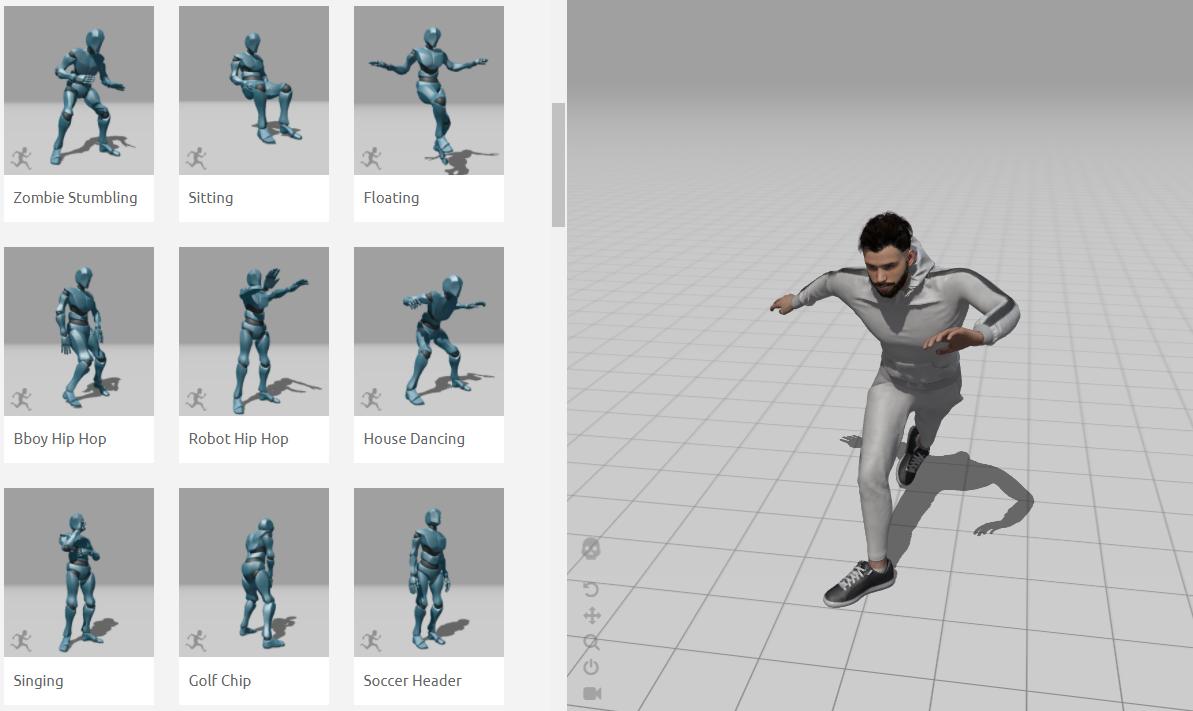
\includegraphics[scale = 0.4]{Mixamo}
    \caption{Servicio de animaciones de Mixamo}
    \label{fig:Mixamo} 
\end{figure} 

Los productos y características de Mixamo son compatibles con todos los paquetes de software 3D, pudiendo realizar una exportación, eligiendo entre varias aplicaciones 3D como: \texttt{Unity, Unreal Engine, Blender} y el conjunto de herramientas de Adobe Creative) entre otros.

Una de las características más sorprendentes de Mixamo, es el \textit{Auto-Rigger}. Ya que ahorras horas de trabajo modelando el personaje y con este sistema, el proceso sucede en cuestión de minutos. Todo lo que se necesita hacer es subir al servidor de Mixamo el personaje 3D (soporta .fbx, .bvh, .zip, obj), seleccionar el número de huesos que mejor se adapte al esqueleto del personaje y esperar que termine el proceso de \textit{rigger}.

Tras completar la fase de modelado, Mixamo ofrece la posibilidad de animar al personaje con movimientos, que permiten, no solo aplicar cualquier animación, sino también personalizarlas, ya que se pueden modificar en tiempo real con el personaje, obteniendo el resultado deseado. Por último, descargarlos en cualquier formato que se necesite (.fbx, .bvh, .dae) y fácilmente se podrá combinar de nuevo en las escenas 3D.

Estas animaciones utilizan una base matemática, lo que facilita su uso para los diferentes personajes que se deseen animar. Tradicionalmente era extremadamente lento, costoso y complicado, lograr modelar personajes 3D con resultados de alta calidad. En cambio, mediante esta técnica, Mixamo intenta reducir los tiempos de desarrollo, pudiendo obtener unas animaciones de calidad, sin la necesidad de contar con altos recursos. 

\section{Hardware empleado}
\label{cap4:sec:hardware empleado}
%---------------------------------------------------------------------
%
%                          capítulo 5
%
%---------------------------------------------------------------------
\chapter{Desarrollo del Proyecto}

\label{cap5:sec:Desarrollo del Proyecto}

Una vez elegida la tecnología y las plataformas que se van a utilizar se empieza a preparar el desarrollo del proyecto. En este capítulo se explicará que libreras y paquete de \texttt{Unity} que se necesitan para tener un entorno de desarrollo potente e innovador. Además, se explicará cuales han sido las metodologías utilizadas para plasmar el proceso seguido para realizar el \textit{Mocap}. El tipo de información guardada, como se ha realizado la grabación de los movimientos captados por los sensores de realidad virtual y cual ha sido la elección para mostrar dicha información.

En la siguiente sección se especificará el proceso realizado para grabar los movimientos capturados, de modo que el profesor obtendrá una visualización directa de cómo ha quedado grabado el movimiento deseado, sin la necesidad de quitarse las gafas de realidad virtual.

Para ofrecer una aplicación dinámica y que el alumno reciba un \textit{feedback} gestual de los movimientos, se ilustra como se diseña e implementan avatares con animaciones en \texttt{Unity}.

De forma sucesiva, se describe el diseño de los escenarios 3D para ubicar a los avatares principales de la aplicación (profesor y alumno). De este modo se han diseñado dos escenarios, uno para grabar y reproducir los movimientos realizados por el profesor dentro de \texttt{VR} y otro en \texttt{AR} donde el alumno podrá visualizar las veces necesarias los movimientos realizado por el profesor.

Posteriormente se elaboran una serie de escenas en \texttt{Unity} que servirán para ilustrar la interfaz para cada una de las aplicaciones (VR y AR). Se ha creado un entorno diferenciado según las necesidades dadas por las diferentes plataformas a desarrollar en el proyecto. Entre estos escenarios las aplicaciones cuentan con las siguientes escenas:

\begin{itemize}
	\item \texttt{VR}: Escena principal de VR, escena de grabación de movimientos, escena de reproducción de los movimientos guardados.
 	\item \texttt{AR}: Escena principal de AR (donde el alumno seleccionará el nivel de aprendizaje) y la escena para realizar el entrenamiento.
\end{itemize}

\section{Investigación para el desarrollo de \textit{Mocap} en Realidad Virtual y Realidad Aumentada}

Parar desarrollar cualquier aplicación en \texttt{Unity} es necesario conocer el contenido que te puede ofrecer la tienda de este \textit{Game Engine}. El \texttt{Asset Store de Unity} es el hogar de una creciente biblioteca de \textit{assets} comerciales y gratuitos creados por \texttt{Unity Technologies} y miembros de la comunidad. Hay una gran cantidad de \textit{assets} disponibles, desde texturas, modelos y animaciones hasta ejemplos de proyectos completos, tutoriales y extensiones del editor. Estos \textit{assets} son accesibles desde una interfaz simple dentro de \texttt{Unity} y son descargados e importados directamente en el proyecto creado.

\subsection{SteamVR}

El primer paquete necesario para poder desarrollar una aplicación de VR en HTC Vice es SteamVR\footnote{\url{https://www.steamvr.com/es/}}. Con este \textit{Asset}(nombre que se le da a los paquetes de Unity) los desarrolladores podemos dirigir una API a la que se pueden conectar todos los auriculares populares de RV para PC. El moderno \texttt{SteamVR Unity Plugin} gestiona tres cosas principales para los desarrolladores: la carga de modelos 3D para los controladores de RV, el manejo de la entrada de esos controladores y la estimación del aspecto de la mano mientras se utilizan esos controladores. Además de gestionar estas cosas, tenemos un ejemplo de Sistema de Interacción para ayudar a poner en marcha una aplicación de VR. Proporcionando ejemplos concretos de interacción con el mundo virtual y las diferentes APIs. 

Además, nos permite acceder a los juegos a través de una interfaz que se proyecta en una habitación de nuestra realidad virtual, que podemos aprovechar para jugar a cualquier juego que tengamos en Steam VR.

Este paquete tiene todo lo necesario para reconocer la conectividad de los dispositivos utilizados en VR y para poder utilizar los datos obtenidos de los sensores colocados en la habitación de juego. 

El Asset nos ofrece una serie de ejemplos básicos para poder comprender mejor el funcionamiento de VR. A su vez, es necesaria la instalación de \texttt{Steam}\footnote{\url{ https://store.steampowered.com}} ya que trae incorporados los drivers imprescindibles para la correcta configuración de los dispositivos utilizados en VR(controles y \textit{trackers}).

Los ejemplos que tiene implementado el paquete de \texttt{SteamVR Plugin} son variados y pueden servir como un buen punto de partida para desarrollar el proyecto. La escena de ejemplo \textit{Interactions\_Example} incluye todos los componentes principales y es un buen lugar para familiarizarse con el sistema. La escena contiene los siguientes elementos:


\begin{itemize}
	\item \texttt{Player}: este \textit{prefab} es el núcleo de todo el sistema. La mayoría de los demás componentes dependen del jugador para estar presente en la escena.
\item \texttt{Teleporting}: el \textit{prefab} \textit{Teleporting} maneja toda la lógica de teletransportación del sistema.
\item \texttt{InteractableExample}: muestra un interacción simple sobre los aspectos básicos para recibir mensajes de las manos y cómo reaccionar ante estas notificaciones.
\item \texttt{Throwables}: muestra cómo se puede utilizar el sistema para interactuar con los objetos y crear diferentes tipos de objetos tirables.
\item \texttt{Skeleton}: diferentes objetos de modelos de mano junto con opciones para determinar a qué mano corresponden del esqueleto.
\item \texttt{Proximity Button}: una tarea común es presionar un botón. Los botones físicos son más satisfactorios de usar que las interfaces planas, pero los sistemas de interacción física pueden volverse complejos rápidamente. Se ha incluido un botón que se puede presionar con solo estar cerca de un controlador.
\item \texttt{Interesting Interactables}: Estos son ejemplos un poco más complejos del uso del sistema \texttt{Skeleton Poser} junto con \texttt{Throwables}. Dependiendo del objeto con el que interactuar obtienes diferentes poses de acción.
\item \texttt{UI}: muestra cómo se manejan las sugerencias en el sistema de interacción y cómo se puede usar para interactuar con los \textit{widgets} de la interfaz, como botones.
\item \texttt{LinearDrive}: este es un objeto un poco más complejo que combina algunas piezas diferentes para crear un objeto animado que se puede controlar mediante interacciones simples.
\item \texttt{CircularDrive}: esto muestra cómo las interacciones se pueden restringir y mapear de manera diferente para realizar movimientos más complejos.
\item \texttt{Longbow}: es uno de los objetos más complejos en el \textit{Asset} y muestra cómo se pueden combinar piezas simples para crear una mecánica de juego completa. 
\end{itemize}

Repasando los diferentes objetos en esta escena de ejemplo te das una amplia idea de la amplitud del sistema de interacción y cómo combinar sus diferentes partes para crear acciones complejas.

Una vez explicado los ejemplos, se elige cuál de ellos se podría utilizar para aprovechar su funcionalidad y tener un apoyo base para el desarrollo del proyecto. Los ejemplos seleccionados serán el \texttt {Player, Skeleton y UI}. Más adelante se explica con más detalle que se utiliza de estos ejemplos.


\subsection{Final IK}

El uso de la realidad virtual presenta muchos desafíos nuevos para el diseño y desarrollo de captura de movimiento, entre ellos el problema de la cinemática inversa (\textit{Inverse Kinematics}). 

La cinemática inversa es la técnica que permite determinar el movimiento de una cadena de articulaciones para lograr que un actuador final se ubique en una posición concreta. El cálculo de la cinemática inversa es un problema complejo que consiste en la resolución de una serie de ecuaciones cuya solución normalmente no es única.\cite{CinematicaInversa}

Este concepto es muy importante para el desarrollo de animaciones en 3D, donde se utiliza para conectar físicamente los personajes del juego en el mundo tridimensional, tales como la sujeción rígida de los pies en un terreno. Una figura animada se modela con un esqueleto de segmentos rígidos conectados con las articulaciones. El problema de cinemática inversa radica en calcular los ángulos de las articulaciones para una pose deseada. A menudo es más fácil para los diseñadores, artistas y animadores definir la configuración espacial de un conjunto sobre las partes móviles, como los brazos y las piernas, en lugar de manipular directamente los ángulos de las articulares. 

Por lo tanto, la cinemática inversa se utiliza en los sistemas \textit{Mocap} para animar las posiciones de las articulaciones. El conjunto de un esqueleto humano se modela como eslabones rígidos conectados por articulaciones que se definen restricciones geométricas. 

Para realizar un movimiento de cualquier extremidad del cuerpo, se requiere el cálculo de los ángulos de las otras articulaciones conectadas con esa parte del cuerpo. Por ejemplo, la cinemática inversa permite mover la mano de un modelo humano 3D con una posición y orientación deseada. Para su correcto funcionamiento es necesario tener un algoritmo que seleccione el ángulo de rotación correcto para cada una de las articulaciones del cuerpo humano, como la muñeca, el codo y los hombros.

Para solventar el problema de la cinemática inversa (véase Figura \ref{fig:IK}) en las articulaciones del cuerpo humano, se estudió una serie de \textit{Assets} capaces de solucionar el problema.

\begin{figure}[h!]
    \centering
    \animategraphics[loop,autoplay,width=0.8\linewidth]{30}{/IK/IK-}{0}{146}
    \caption{Diferencia entre \textit{Forward Kinematics e Inverse Kinematics}}
    \label{fig:IK}  
\end{figure}

La primera elección fue UMotion \footnote{\url{ https://www.soxware.com/umotion/}}, ya que se trata de un editor de animación que ofrece potentes herramientas y flujos de trabajo dentro de Unity. La creación de animaciones en la misma aplicación y situación en la que se van a utilizar simplifica todo el flujo de trabajo acelerando el desarrollo del proyecto. 

El problema surgió cuando se intentan asignar los diferentes componentes de VR dentro del \textit{Asset}, no era posible realizar dicha acción, no admitía VR, por lo que fue descartada esta opción.

\vspace{1cm}
Actualmente no hay muchas soluciones \textit{IK} de cuerpo completo disponibles que cumplan con los requisitos muy específicos del desarrollo en realidad virtual.

Además de la precisión y la calidad general de la cinemática inversa, también es vital que el \textit{Asset} sea altamente eficiente y eficaz, ya que la realidad virtual tiene una gran carga de CPU y GPU. 

Por lo tanto, la realidad virtual requiere que \textit{IK} se resuelva no solo en alta frecuencia, sino también en alta calidad: todo se vuelve observable con gran detalle y en primera persona más aun, ya que incluso debe estar a la altura de la comparación con la realidad.

Teniendo en cuenta todo esto, se optó por la solución \texttt{Final IK} \footnote{\url{http://root-motion.com/}}, la cual cumplía con todos estos requisitos, incluyendo la compatibilidad con VR. 

\subsection{ARCore}



%---------------------------------------------------------------------
%
%                          bibliografia.tex
%
%---------------------------------------------------------------------


\printbibliography





\end{document}